\documentclass[12pt, a4paper]{article}
\usepackage[utf8]{inputenc}
\usepackage{graphicx}
\graphicspath{ {images/} }
\usepackage{hyperref}
\usepackage{xcolor}

\title{\emph{Computer Science Resources }}
\author{Written by Volunteers}
\date{April 19, 2021}

\begin{document}

\maketitle
\section*{License}
\paragraph{}
This work is released under the \href{https://creativecommons.org/share-your-work/public-domain/}{\textcolor{blue}{CC0}} License. for getting more information about this License please refer to the creative commons \href{https://creativecommons.org}{\textcolor{blue}{website}}.\\
\\
\includegraphics[scale=0.4]{cc-zero}

\paragraph{}
The List order isn't important. I used numbers to make it easier for you to find each topic. for example DSA is listed Before C , but it is better to learn both of them with \textbf{each other}.

\newpage
\section*{Important Notes :}
\paragraph{}
\emph{Mathematics} especially \emph{\textbf{Discrete Mathematics \footnote{ A branch of Mathematics that studies discrete structures such as Integers , Graphs and statements in Logic}}} is a \textbf{must} for every Software Engineer. So you must have enough knowledge to solve \emph{complex problems} in Software Engineering.

\paragraph{}
Always find \emph{every book's \textcolor{red}{Errata} \footnote{A list of errors in a printed work discovered after printing and shown with corrections}} that \emph{you want to read} , via the \emph{Internet}.

\subsection*{This books are popular for \emph{Discrete Mathematics} :}
\paragraph{}
\emph{Discrete Mathematics and Its Applications} written by \emph{Kenneth H.Rosen} is a good book for learning Discrete Mathematics , but it's a \textbf{time-consuming} process to read this book.
\paragraph{} 
You can read \emph{Introductory Discrete Mathematics} , a book which is written by \emph{V.K Balakrishnan} that is a good starting point for \textbf{full beginners} in Discrete Mathematics.\\

\begin{center}
	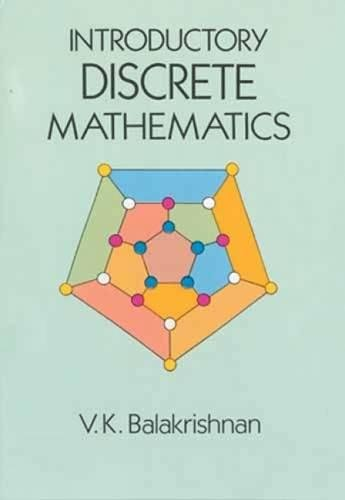
\includegraphics[scale=0.5]{IDM.jpg}
\end{center}


\newpage
\section*{Recommendation :}
\paragraph{}
I \emph{recommend} you to read these books to learn \emph{Discrete Mathematics} :
\begin{enumerate}
	\item Elements of Discrete Mathematics , \emph{\large{Chung Laung Liu}}
	\item Discrete Mathematics with Applications , \emph{\large{Susanna S.Epp}}
\end{enumerate}

\paragraph{}
\href{https://ocw.mit.edu/courses/electrical-engineering-and-computer-science/6-042j-mathematics-for-computer-science-spring-2015/}{\textcolor{blue}{\emph{Mathematics for Computer Science}}} by \emph{MIT OCW} is a good course , that also provides a practical \href{https://courses.csail.mit.edu/6.042}{\textcolor{blue}{\emph{reading material}}}.

\paragraph{}
\emph{Mathematics : A Discrete Introduction} is another \emph{efficient} book.

\paragraph{}
Also , i \emph{recommend} you to read these books for \textbf{\emph{Linear Algebra}} :
\begin{enumerate}
	\item Introduction to Linear Algebra , \emph{\large{Gilbert Strang}}
	\item Linear Algebra Done Right ,  \emph{\large{Sheldon Axler}}
	\item Linear Algebra Done Wrong , \emph{\large{Sergei Treil}\\}
	\item Finite Dimensional Vector Spaces , \emph{\large{Paul Halmos}}
	\item Linear Algebra Problem Book , \emph{\large{Paul Halmos}}
	\item Advanced Linear Algebra , \emph{\large{Steven Roman}}
\end{enumerate}
\paragraph{}
The \emph{Linear Algebra step by step} is another good book for this field.

\paragraph{}
For \textbf{\emph{Calclus}} , i think these books are \emph{efficient} :
\begin{enumerate}
	\item Calculus of one Variable ,  \emph{\large{Joseph W. Kitchen}}
	\item Calculus , Volume 1 , \emph{\large{Tom M.Apostol}}
	\item Calculus , Volume 2 , \emph{\large{Tom M.Apostol}}
	\item Calculus , \emph{\large{Spivack}}
\end{enumerate}
\paragraph{}
I \emph{recommend} you to \emph{supplement} them with \emph{these} courses :

\begin{enumerate}
	\item \href{https://ocw.mit.edu/courses/mathematics/18-014-calculus-with-theory-fall-2010/}{\emph{\textcolor{blue}{Single Variable Calculus}}}
	\item \href{https://ocw.mit.edu/courses/mathematics/18-024-multivariable-calculus-with-theory-spring-2011/}{\emph{\textcolor{blue}{Multivariable Calculus with Theory}}}
\end{enumerate}
\paragraph{}
Or you can try any other course that is \emph{related} to this subject.

\newpage
\paragraph{}
Finally for \textbf{\emph{Probablility} \& \emph{Statistics}} read these books :
\begin{enumerate}
	\item Introduction to Probability , \emph{\large{Blitzstein and Hwang}}
	\item Introduction to Probability, \emph{\large{Bertsekas  and Tsitsiklis}}
	\item \emph{Introduction to Probability, Statistics, and Random Processes\\}
	\item The Art of Probability , \emph{\large{Richard W. Hamming}}
	
	 \item An Introduction to Probability Theory and Its Applications, \emph{\large{Vol 1}}
	 \item An Introduction to Probability Theory and Its Applications, \emph{\large{Vol 2}}
\end{enumerate}

\subsubsection*{Important Notes :}
\paragraph{}
\emph{The Art of Probability} ,  can be used as a supplement for the \emph{first 3 books}.

\paragraph{}
The \emph{last 2 books} \textbf{are not easy to read} for \emph{\large{beginners}}.

\paragraph{}
These books are \emph{\large{specialized}} for \textbf{\emph{Statistics}} :
\begin{enumerate}
	\item \emph{All of Statistics : A Concise Course in Statistical Inference}
	\item Theoretical Statistics , \emph{\large{D.R. Cox and D.V. Hinkley}} 
\end{enumerate}

\section*{Additional Resources :}
\begin{enumerate}
	\item \href{https://www.3blue1brown.com}{\emph{\textcolor{blue}{\large{3Blue1Brown}}}}
	\item \href{https://www.coursera.org/specializations/mathematics-machine-learning}{\emph{\textcolor{blue}{Mathematics for Machine Learning Specialization}}}
	\item \emph{\large{Concrete Mathematics}}
\end{enumerate}

\newpage
\section{Introduction to Computer Science}
\subsection*{\href{https://cs50.harvard.edu/college/2021/spring/}{\textcolor{blue}{CS50}} , harvard university course \emph{(week 1-6)}}
\paragraph{}
this course is an introductory course to computer science.\\

\section{Python 3 \emph{Basics}}
\subsection*{Python \href{https://www.edx.org/course/programming-for-everybody-getting-started-with-pyt}{\textcolor{blue}{for Everybody}}
and \href{https://www.edx.org/course/python-data-structures}{\textcolor{blue}{Data structures}} , Edx}
\paragraph{}
these 2 courses are good resources for learning Python 3 for beginners.
\subsection*{Python Crash Course , Nostarch Press\\}

\section{Data Structures and Algorithms (DSA)}
\subsection*{Grokking Algorithms}
\paragraph{}
This is a well written book for beginners. it covers the most useful \emph{Data Structures} and \emph{Algorithms} , but it has its own \textbf{limits}.  

\subsection*{Princeton and Stanford Courses}

\begin{enumerate}
\item Algorithms , \href{https://www.coursera.org/learn/algorithms-part1}{\textcolor{blue}{Part I}}
\item Algorithms , Design and Analysis \href{https://www.edx.org/course/algorithms-design-and-analysis}{\textcolor{blue}{Part 1}}
\item Algorithms , Design and Analysis \href{https://www.edx.org/course/algorithms-design-and-analysis-part-2-2}{\textcolor{blue}{Part 2}}
\item Algorithms , \href{https://www.coursera.org/learn/algorithms-part2}{\textcolor{blue}{part 2}}
\end{enumerate}

\subsection*{Introduction to Algorithms ({Reference})}
\subsection*{The Algorithms Design Manual (Optional)}
\paragraph{}
After learning the concpets , read \emph{Algorithms in C} by Robert Sedgewick or any other book (\emph{The Algorithm Design Manual} , $\dots$) for \textbf{implementing} Algorithms in C.

\section{C Programming Language}
\subsection*{C Programming : A Modern Approach}
\paragraph{}
An excellent book for Beginners.
\subsection*{Pointers on C}
\paragraph{}
Another excellent C programming book that is very helpful for everyone who wants to learn \textbf{C pointers}.
\subsection*{C Programming Language (K\&R)}
\paragraph{}
A classic book written by Dennis Ritchie and Brian Kernighan.
\subsection*{C in a Nutshell}
\paragraph{}
A great book for Modern C. you can also check \textbf{modern C} book that is written by \emph{jens Gustedt}.

\section{Theory of Computation}

\subsection*{\emph{* Micahel Sipser and Dexter C.Kozen *}}
\subsubsection*{Introduction to the Theory of Computation (Michael Sipser)}
\subsubsection*{Automata and Computability (Dexter C.kozen)}
\paragraph{}
Reading these two books , give you a complete understanding. You can also check other resources like \textbf{stanford} course and \textbf{Cindrella Book}.

\subsection*{\emph{* Additional Resources *}}
\subsubsection*{\href{https://www.edx.org/course/automata-theory}{\textcolor{blue}{Automata Theory}} , Stanford university Course}
\subsubsection*{\scalebox{0.8}{Introduction to Automata Theory , Language , and Computation (1st and 2nd Edition) (Reference)}}
\paragraph{}
most of the readers of this book said that the \emph{3rd Edition} doesn't have the helpful exercises that was present in the \emph{1st and 2nd Editions}.

\section{Compilers}
\subsection*{\emph{* introduction *}}
\subsubsection*{\href{https://www.edx.org/course/compilers}{\textcolor{blue}{Compilers}} , Stanford university Course}
\subsection*{\emph{* Concepts *}}
\subsubsection*{Compilers : Principles , Techniques and Tools (2nd Edition)}
\paragraph{}
Also known as \emph{Purple Dragon Book} , it is the \textbf{most recent} Book for Compilers written by Aho. But some concepts are better explained in \emph{Red} and \emph{Green Dragon} Books.
\subsubsection*{\scalebox{0.85}{Compilers : principles , Techniques and Tools (\emph{Red Dragon Book}) (Reference)}}
\subsubsection*{Principles of Compiler Design (Green Dragon Book) (Reference)\\}
\subsection*{\emph{* Implementation *}}
\subsubsection*{\href{https://holub.com/compiler/}{\textcolor{blue}{Compiler Design in C}} (Allen Holub)}
\subsubsection*{Brinch hansen on pascal compilers}

\section{Digital Logic / Digital Design}
\subsubsection*{\emph{Digital Design and Computer Architecture} by Harris \& Harris }
\subsubsection*{\emph{Digital Circuits and Design} by S. Salivahanan \& S. Arivazhagan}
\subsubsection*{\textit{Digital Design Principles and Practices} (\emph{Reference})}


\section{Computer Architecture}
\subsection*{\emph{* Books *}}
\subsubsection*{\small{Computer Organization and Design : The Hardware/Software Interface}}
\subsubsection*{Computer Architecture : A Quantitative Approach}
\subsection*{\emph{* Courses *}}
\subsubsection*{\href{https://www.coursera.org/learn/comparch}{\emph{\textcolor{blue}{Computer Architecture}}} , Princeton university course}
\subsubsection*{\emph{Onur Mutlu} Lectures}
\newpage
\subsection*{\emph{* Additional *}}
\subsubsection*{\scalebox{1}{Structured Computer Organization by Andrew Tanenbaum \& Todd Austin}}
\paragraph{}
This book is recommended to \emph{\textbf{beginners}}.
\subsubsection*{The university of \emph{Wisconsin-Madison} recommendation}
\url{http://pages.cs.wisc.edu/~arch/www/books.html}\\

\section{Operating Systems}
\subsection*{\emph{* Concepts *}}
\subsubsection*{Operating System Concepts}
\subsubsection*{Modern Operating Systems (Reference)}
\subsection*{\emph{* Examples *}}
\subsubsection*{The Design of Unix Operating System by Maurice Bach}
\paragraph{}
You can also read \href{https://nostarch.com/howlinuxworks3}{\emph{\textcolor{blue}{How Linux Works : What Every Superuser Should Know}}} or any other book about this subject.
\subsection*{\emph{* Implementation *}}
\subsubsection*{Operating Systems : Design and Implementation\\}

\section{Shell Scripting}
\subsection*{The Linux Command Line}
\subsection*{\scalebox{0.8}{Unix and Linux System Administration Handbook (4th \& 5th Edition) (Reference)}}
\paragraph{}
Some concepts aren't coverd in the \emph{5th} Edition (Latest Edition) , but covered in the \emph{4th Edition}. 

\section{Computer Networking (\emph{Basics})}
\subsection*{\emph{* Introduction *}}
\subsubsection*{\href{https://www.edx.org/course/introduction-to-networking}{\textcolor{blue}{Introduction to Networking}} , NYU course}
\subsection*{\emph{* Concepts *}}
\subsubsection*{Computer Networks by Andrew S. Tanenbaum}
\subsubsection*{\scalebox{1}{TCP/IP Illustrated Vol. 1 : The Protocols by \emph{W. Stevens} (1st Edition)}}
\paragraph{}
The \textbf{2nd} Edition of TCP/IP Illustrated vol 1 isn't \emph{Ideal} for \textbf{Beginners} and Consists of many \emph{Mistakes}. So the \textbf{1st} Edition is better for this purpose.

\section{Game Theory}
\subsection*{\emph{* Introduction  *}}
\subsubsection*{A Brief Introduction to the basics of Game Theory}
\scalebox{1.2}{\url{https://papers.ssrn.com/sol3/papers.cfm?abstract_id=1968579}}

\subsection*{\emph{* Courses *}}
\subsubsection*{\href{https://www.coursera.org/learn/game-theory-1}{\textcolor{blue}{Game Theory}} , Stanford university course}
\subsubsection*{\href{https://www.coursera.org/learn/game-theory-introduction}{\textcolor{blue}{Welcome to Game Theory}} , Tokyo university course}
\subsubsection*{\href{http://timroughgarden.org/f13/f13.html}{\emph{\textcolor{blue}{Algorithmic Game Theory}}} , Tim Roughgarden \emph{(fall 2013)}}

\subsection*{\emph{* Books *}}
\subsubsection*{Twenty Lectures on Algorithmic Game Theory}
\subsubsection*{Algorithmic Game Theory}
\scalebox{1}{\url{https://www.cs.cmu.edu/~sandholm/cs15-892F13/algorithmic-game-theory.pdf}}
\subsubsection*{Multiagent Systems}
\scalebox{1.2}{\url{http://www.masfoundations.org}}
\paragraph{}
\scalebox{1}{These resources don't have special \textbf{prerequisites} except a basic knowledge in :}

\begin{large}
\begin{center}
	\emph{Probability} , \emph{Calculus} , \emph{Algorithms}
\end{center}	
\end{large}


\newpage
\section{Additional Resources}
\subsection*{\emph{* Programming *}}
\subsubsection*{Structure and Interpretation of Computer Programs (\href{https://mitpress.mit.edu/sites/default/files/sicp/index.html}{\textcolor{blue}{SICP}})}
\paragraph{}
An \emph{Introduction} to Programming for \textbf{Experts}.
\subsubsection*{Standard C Library}
\subsubsection*{\scalebox{0.8}{Advanced Programming in the UNIX Environment, 3rd Edition by W. Stevens and Stephen Rago}}
\subsection*{\emph{* Computer Networking *}}
\subsubsection*{\scalebox{0.8}{The TCP/IP Guide : A Comprehensive , Illustrated Internet Protocols Reference} \scalebox{0.9}{(Reference)}}
\paragraph{}
It is a good book as a \emph{Reference} , but the Implementations aren't useful nowadays , because the book was published in \textbf{2005}.
\subsubsection*{TCP/IP Illustrated, Vol. 2 : The Implementation (Reference)}
\paragraph{}
Another good book for studying \emph{Computer Networking} , it is outdated (\textbf{Published 1995}) but explains concepts very well.

\begin{huge}
\section*{Good Luck}
\paragraph{}
\end{huge}

\end{document}
